\documentclass[final,hyperref={pdfpagelabels=false}]{beamer}

\usepackage{macros}
\usepackage{fontawesome5}
\usepackage{hyperref}

\usefolder{../}
\usetheme{CS}

%%%%%% To change the theme color, uncomment the following lines and set your own color. %%%%%%
%%%%%%%% You can also directly modify the colors in the file beamercolorthemeCS.sty %%%%%%%%
%
% \definecolor{mycolor}{rgb}{0.61, 0.42, 0.61}
\definecolor{mycolor}{RGB}{85, 40, 111}
\definecolor{headercolor}{RGB}{11, 9, 10}
\definecolor{blockbgcolor}{RGB}{245, 243, 244}
%\colorlet{codebg}{mycodecolor}
% 
\setbeamercolor{structure}{bg = mycolor}
\setbeamercolor{title page}{fg = mycolor}
\setbeamercolor{alerted text}{fg = mycolor, bg = main}
\setbeamercolor{block title example}{fg = mycolor}
\setbeamercolor{block body}{bg = blockbgcolor}
\setbeamertemplate{bibliography item}{\insertbiblabel}

\usepackage{times}
\usepackage{amsmath,amsthm, amssymb, latexsym}
\usepackage{xcolor}
\boldmath
\usepackage[english]{babel}
\usepackage[latin1]{inputenc}
\usepackage[orientation=landscale, size=a4, scale=1.5, debug]{beamerposter}

\usepackage{graphicx}
\usepackage{subcaption}
\usepackage{float}
\usepackage{tipa}

\usepackage{xspace}
\usepackage[inline]{enumitem}

\usepackage{tikz}
\usetikzlibrary{tikzmark}

%% Fonts used in the template cannot be substituted; margin 
%% adjustments are not allowed.
    
% \newcommand\ytl[2]{
% \parbox[b]{8em}{\hfill{\color{violet}\bfseries\sffamily #1}~$\cdots$~}\makebox[0pt][c]{$\bullet$}\vrule\quad \parbox[c]{5cm}{\vspace{7pt}\color{darkgray}\raggedright\sffamily #2.\\[7pt]}\\[-3pt]}

%Use arabic numbers instead of letters for marking the footnote -VP
\renewcommand{\thempfootnote}{\arabic{mpfootnote}}
%Remove the line separating the footnote -VP
%\renewcommand*\footnoterule{}

\usepackage[scale=1.6]{ccicons}

\def\q{\textquotesingle}

  \graphicspath{{figures/}}
  
  \title{The Transparent CHI Paper}
  \subtitle{Cheat Sheet}

  \begin{document}
  
  \begin{frame}[fragile]{} 
    \vfill
    \begin{columns}[t]
      \begin{column}{.4\linewidth}
        \maketitle
        % !TEX root = 1_Main.tex

%%% This is all first draft/getting ideas into place. -- Jan
\begin{block}{What is Transparency}
   \begin{quote}
       Having one\textquotesingle s actions open and accessible for external evaluation. Transparency pertains to researchers being honest about theoretical, methodological, and analytical decisions made throughout the research cycle.
   \end{quote} 
   Framework for Open and Reproducible Research Training (\href{https://forrt.org/glossary/transparency/}{FORRT.org})  
  
  \blocksubtitle{Why be transparent?}
  \begin{itemize}
  \item Help readers and reviewers understand your work
  \item Helps you stay on top of your work
  \item Prevent mistakes
  \item Work faster
  \item Create better research. 
  \item Increase citations and promote reuse
  \end{itemize}  
  Being transparent benefits you as much as others~\footnotemark[1]. 
  %\cite{markowetz_five_2015}:
  
%   \begin{itemize}
%       \item Work aimed to be made transparent has to be kept orderly and readable. This is easier for everyone (yourself and others) to follow and understand. 
%       \item Well kept materials are more easily reused by others and yourself
%       \item Transparent materials and data allow reviewers to more easily follow your argument
%       \item Transparent data/research materials can be checked more easily for mistakes, making it easier to catch them before publication
%   \end{itemize}


  %\blocksubtitle{Is transparent research inherently better?}
  %\begin{itemize}
   %   \item Not necessarily, \textbf{but} 
      %\item going through pre-registration forces you to think about your study before you commit 
     % \item keeping track of your work prevents mistakes
     % \item making data and materials available increase citation counts
      
      
 %     (e.g., what is my dependent variable, how do I measure it). This can help you keep track of your works intended core idea and save you from uncomfortable surprises at a point where you can no longer change certain things (e.g., after data collection).
 % \end{itemize}
 
% \blocksubtitle{\faIcon{skull-crossbones}  What do we want to avoid? \faIcon{skull-crossbones}}
  
%   \begin{itemize}
%       \item Questionable Research Practices (QRP) e.g.,
%       \item HARKing (Hypothesizing After Result Known)
%       \item p-hacking 
%       \item cherry-picking
%       \item data dredging
%   \end{itemize}

 
%  \blocksubtitle{How to be Transparent without (much) Extra Work?}
%  \begin{itemize}
%    \item Tacking on open science practices at the end of a project %often feels like extra work
%    \item Integrate transparency from day one of your research (check the timeline on the back).
%  \end{itemize}
%   Open Science practices can seem like extra work, particularly if you when having to implement them into an existing project. However, when you are intending to be transparent at publication from the start, the required work can be (almost) seemingly integrated into your normal work. Subsequently it does not require much more time or effort during any single step of research.
  
 
  
  \blocksubtitle{What should I make transparent?}
  Almost any researcher can integrate transparent practices. However:
\begin{itemize}
      \item Keep in mind participant safety and rights 
      \item Some data cannot be shared safely
      \item Use data availability statement to report what can and can't be shared
  \end{itemize} 
Even if data must be kept private, share what materials you can (interview questions, analysis code, or other materials). 
% and use a \href{https://www.cambridge.org/core/services/authors/open-data/data-availability-statements}{data availability statement} to transparently report what you can and can\textquotesingle t share.
\end{block}

\begin{block}{Inspiration/Examples}
\blocksubtitle{Papers}
Broman, Wu (2018). Data organization in spreadsheets \\ \href{https://peerj.com/preprints/3183/}{peerj.com/preprints/3183}
\\ Wickham (2014). Tidy Data. \href{http://www.jstatsoft.org/v59/i10/}{jstatsoft.org/v59/i10}
\\ Wilson, G. et al (2017). Good enough practices in scientific computing \href{https://doi.org/10.1371/journal.pcbi.1005510}{doi.org/10.1371/https://doi.org/10.1371/journal.pcbi.1005510}
\blocksubtitle{Organizations}
 Center for Open Science \href{https://www.cos.io/}{cos.io}
\\ The Alliance for Open Scholarship \href{https://www.all4os.org/}{all4os.org}
\\ Project TIER \href{https://www.projecttier.org/}{projecttier.org}
\\ Framework for Open and Reproducible Research Training \href{https://forrt.org/glossary/transparency/}{FORRT.org}
\\ FOSTER Open Science \href{https://www.fosteropenscience.eu/}{fosteropenscience.eu}

\end{block}

\footnotetext[1]{Markowetz, F. (2015). Five selfish reasons to work reproducibly. Genome biology, 16(1), 1-4.}
      \end{column}
      
      \begin{column}{.6\linewidth}
    % !TEX root = 1_Main.tex

\begin{block}{Common tools}
\vskip-2ex
  \begin{columns}[t]\hfill\hfill\hfill
    \begin{column}{.45\linewidth}
 \begin{subblock}{\faIcon{folder} \hfill Data and File Organization\hfill \faIcon{folder-open}}
%TIER protocol \href{https://www.projecttier.org/tier-protocol/protocol-4-0/}{ProjectTIER.org}

Research Data Alliance \href{rd-alliance.org/}{rd-alliance.org/}
    \vskip-1ex
  \end{subblock}
  
  \begin{subblock}{\faDatabase \hfill Data Repositories \hfill \faDatabase}
 \begin{itemize}
     \item \textbf{Open Science Framework (OSF)}
     \item Zenodo
     \item Harvard Dataverse
     \item ICPSR
    %  \item Dryad
    %  \item Figshare
    %  \item Vivli

 \end{itemize}
    \vskip-1ex
  \end{subblock}
  
  \begin{subblock}{\faIcon{table} \hfill Paper Repositories \hfill \faIcon{table}}
 \begin{itemize}
     \item \textbf{Open Science Framework (OSF)}
     \item arXiv
 \end{itemize}
    \vskip-1ex
  \end{subblock}  

  \begin{subblock}{\faSearch \hfill Make your work findable\hfill \faSearch}
Ensure it is indexed and has a unique identifier. Try CrossRef, ORCiD, doi.

    \vskip-1ex
  \end{subblock}  
  
  \begin{subblock}{\faIcon{id-badge}\hfill Licenses\hfill \faIcon{id-badge}}
 \begin{itemize}
\item CC-BY \href{https://creativecommons.org/about/cclicenses/ 
}{creativecommons.org}
\item MIT \href{https://mit-license.org/ }{mit-license.org}
 \end{itemize}
    \vskip-1ex
  \end{subblock}  

  \end{column}\hfill
   \begin{column}{.45\linewidth}

\begin{subblock}{\faIcon{file-alt} \hfill Analysis tools\hfill \faIcon{file-alt}}
Open source software is more transparent \\ \vspace{0.5em}
 \faIcon{r-project} R \href{https://www.r-project.org/}{r-project.org}
\\ \faIcon{python} Python \href{https://www.python.org/}{python.org}
\\ JASP \href{https://jasp-stats.org/}{jasp-stats.org} \\ \vspace{0.5em}
...but, you can be transparent with closed-source software, too!
  \end{subblock}
   
\begin{subblock}{\faIcon{file-alt}\hfill Literate programming\hfill \faIcon{file-alt}}
Mixing text and code helps document your work \\ \vspace{0.5em} \faIcon{r-project}, \faIcon{python}, \faIcon{file-code}  Quarto \href{https://quarto.org/}{quarto.org}
\\ \faIcon{r-project} RMarkdown \href{https://rmarkdown.rstudio.com/}{rmarkdown.rstudio.com}
\\ \faIcon{python} Jupyter Notebooks \href{https://jupyter.org/
}{jupyter.org}
  \end{subblock}

  \begin{subblock}{\faIcon{file-code}\hfill Code Repositories\hfill \faIcon{file-code}}
\begin{itemize}
    \item GitHub \faIcon{github}
    %\item Open Science Framework (OSF)
    \item Zenodo
    \item GitLab \faIcon{gitlab}
    \item Bitbucket \faIcon{bitbucket}

\end{itemize}
  \end{subblock}
  \end{column}\hfill\hfill\hfill

  \end{columns}
   ...there are many more resources in all these categories! Pull requests welcome.   
   
% \begin{center}
%     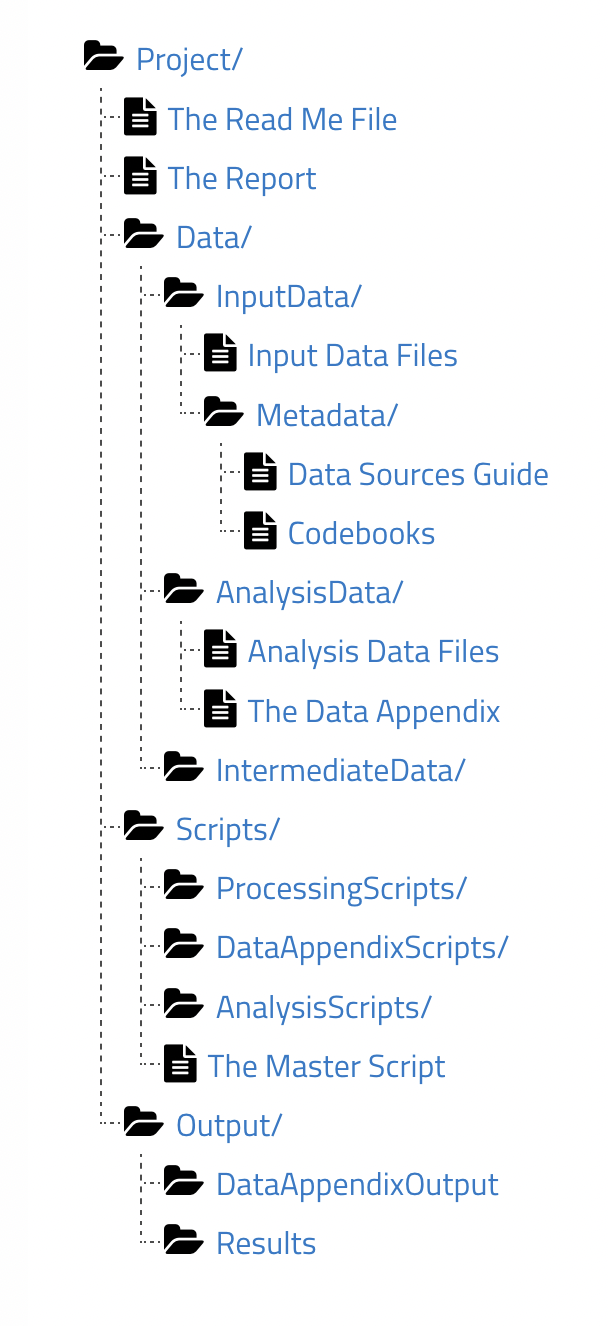
\includegraphics[width=0.6\textwidth]{img/TIER_protocol.png} \\
%     TIER Protocol ProjectTIER.org
% \end{center}

\end{block}
        % !TEX root = base-r.tex

\begin{block}{Checklist}
Use this overview to keep track of what you did. Ignore the points not applicable to your project.
\begin{itemize}
\item[$\square$]
Ethics approval granted
\item[$\square$]
(Confirmatory) User study preregistered
\item[$\square$]
Participant consent for open data sharing collected
\item[$\square$]
Data collection process documented
\item[$\square$]
De-Identified Data and data documentation (e.g., data dictionary) is uploaded to a repository that gives unique identifiers (e.g., DOI).

\item[$\square$]
Source code for data analysis cleaned up and commented
\item[$\square$]
Methodology comprehensibly described
\item[$\square$]
Citation list is clear and complete (including used software packages)
\item[$\square$]
All contributions are acknowledged

\item[$\square$]
Supplementary material documented and uploaded
\item[$\square$]
Repository given an open licence (e.g., \href{https://creativecommons.org/licenses/by/4.0/}{CC-BY})
\item[$\square$] Add a \href{https://www.cambridge.org/core/services/authors/open-data/data-availability-statements}{data availability statement}
\item[$\square$]
Paper published open access 
\end{itemize}
\end{block}

% \begin{block}{\hyperlink{https://forrt.org/glossary/}{Go to FORRT Glossary}}
% \end{block}

      \end{column}
     \end{columns}
    \vfill
  \end{frame}
\clearpage  
  \begin{frame}[fragile]{}
    \begin{columns}[t]
      \begin{column}{0\linewidth}
      \end{column}
            
      \begin{column}{\linewidth}
              % !TEX root = 1_Main.tex

\begin{block}{Timeline}
Fill in the blanks with your target deadlines. If a particular step does not apply to your work, feel free to cross it out. 
\begin{table}[]
\Large
\color{darkgray}
\begin{tabular}{rlll}
\multicolumn{1}{c}{\textcolor{headercolor}{\textbf{TIMELINE}}} & \multicolumn{2}{c}{\textcolor{headercolor}{\textbf{YOUR ACTION ITEMS}}} & \textcolor{headercolor}{\textbf{RESOURCES}}\\
& & & \\
\multirow{2}{*}{\color{violet}\framebox(80, 25){} $\cdots$\makebox[0pt][c]{$\bullet$}}  &\multirow{2}{*}{\textbf{Ethics Approval}} &  $\cdot$ collect data sharing & [Check your universities guidelines]\\
 & & consent& \\
 %& & & \\
\multirow{2}{*}{\color{violet}\framebox(80, 25){} $\cdots$\makebox[0pt][c]{$\bullet$}} & \multirow{2}{*}{\textbf{Preregistration}} & Check if a Preregistration could be beneficial for your work. &
    \href{https://aspredicted.org/}{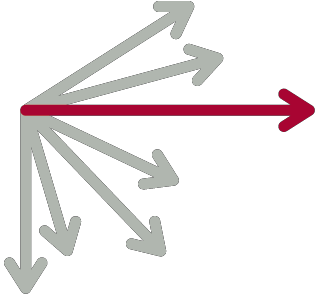
\includegraphics[width=0.8cm]{img/aspredicted_penn_wharton.png}}  
\href{https://aspredicted.org/}{AsPredicted.org}\\
 & & If yes, Preregister & \href{https://osf.io/registries}{
\includegraphics[width=0.8cm]{img/osf registries.png}}  
\href{https://help.osf.io/article/345-create-registrations}{OSF Guide and templates}  \\
  & & & \\
  \multirow{2}{*}{\color{violet}\framebox(80, 25){} $\cdots$\makebox[0pt][c]{$\bullet$}} &\textbf{Data Collection} &  $\cdot$ deidentify/anonymize data, &  \href{https://edps.europa.eu/system/files/2021-04/21-04-27_aepd-edps_anonymisation_en_5.pdf}{
\includegraphics[width=0.75cm]{img/anonymise_data.png}} 
  \href{https://edps.europa.eu/system/files/2021-04/21-04-27_aepd-edps_anonymisation_en_5.pdf}{How To}\\
 \color{violet} & \textbf{and Organization} & choose a non-proprietary file format (e.g., csv) &  \\
 & &$\cdot$ create a data dictionary & \href{https://github.com/yvonnejansen/posture/blob/master/data/exp1_column-description.csv}{
\includegraphics[width=0.75cm]{img/data_dictionary.png}} \href{https://github.com/yvonnejansen/posture/blob/master/data/exp1_column-description.csv}{Check Example}\\
  & & & \\
\multirow{2}{*}{\color{violet}\framebox(80, 25){} $\cdots$\makebox[0pt][c]{$\bullet$}} &\textbf{Data Analysis} &  $\cdot$ clean, executable, and & \href{https://www.r-project.org/}{
\includegraphics[width=0.95cm]{img/Rlogo.png}}  \href{https://www.r-project.org/}{R} \quad \href{https://www.python.org/}{
\includegraphics[width=0.75cm]{img/python_logo.jpg}}  \href{https://www.python.org/}{Python} \quad \href{ https://jasp-stats.org/}{
\includegraphics[width=0.8cm]{img/JASP_logo.png}}  \href{ https://jasp-stats.org/}{JASP}\\
 & & commented code/script & \\
 & & &  \\
%  & & & \\
\multirow{2}{*}{\color{violet}\framebox(80, 25){} $\cdots$\makebox[0pt][c]{$\bullet$}} &\textbf{Supplementary} &  Add to a repository: &  \href{https://zenodo.org/}{
\includegraphics[width=1.5cm]{img/zenodo.png}}  \href{https://zenodo.org/}{Zenodo.org}\\
 & \textbf{Material} & $\cdot$ data,  &
 \href{https://dataverse.harvard.edu/}{
\includegraphics[width=1.5cm]{img/harvard_dataverse.png}} \href{https://dataverse.harvard.edu/}{Harvard Dataverse}\\
  & & $\cdot$ study protocols,  & \href{https://osf.io/}{
\includegraphics[width=0.8cm]{img/osf registries.png}}   \href{https://osf.io/}{OSF Repository}\\
 & & $\cdot$ analysis scripts, &
  \href{https://github.com/}{
\includegraphics[width=0.8cm]{img/GitHub-Mark-64px.png}} \href{https://github.com/}{GitHub}
  \\ %\href{https://www.icpsr.umich.edu/web/pages/}{ICPSR}
  & & $\cdot$ videos, and &  \href{https://gitlab.com/}{
\includegraphics[width=0.8cm]{img/gitlab-logo-500.png}} \href{https://gitlab.com/}{GitLab}\\
& & $\cdot$ anything else relevant to you. & \\
& & & \\
\multirow{2}{*}{\color{violet}\framebox(80, 25){} $\cdots$\makebox[0pt][c]{\faTrophy}} & &  &\\
& \multicolumn{2}{c}{
\includegraphics[width=0.75cm]{img/star (1).png} \color{violet}YOU DID IT! 
\includegraphics[width=0.75cm]{img/star (1).png}}& \\
\end{tabular}
\end{table}



% \begin{table}
% %\caption{Fill in the blanks with your target deadlines}
% \centering
% \begin{minipage}[t]{.99\linewidth}
% \color{gray}
% \rule{\linewidth}{1pt}
% \ytl{\framebox(60,20){}}{Include Data Sharing Statement in the Ethics Approval}
% \ytl{\framebox(60,20){}}{Preregistration}
% \ytl{\framebox(60,20){}}{Data Collection and Organization}
% \ytl{\framebox(60,20){}}{Deidentification of Participant Data}
% \ytl{\framebox(60,20){}}{Create a Data Dictionary}
% \ytl{\framebox(60,20){}}{Analyse Data}
% \ytl{\framebox(60,20){}}{Clearly Commented Code}
% \ytl{\framebox(60,20){}}{Submit data to a FAIR repository}
% \ytl{\framebox(60,20){}}{Submit supplementary material to a repository}
% \bigskip
% \rule{\linewidth}{1pt}%
% \end{minipage}%
% \end{table}

\end{block}

      \end{column}
     \end{columns}
   \end{frame}

\end{document}